% This is samplepaper.tex, a sample chapter demonstrating the
% LLNCS macro package for Springer Computer Science proceedings;
% Version 2.21 of 2022/01/12
%
\documentclass[runningheads]{llncs}
%
\usepackage[T1]{fontenc}
% T1 fonts will be used to generate the final print and online PDFs,
% so please use T1 fonts in your manuscript whenever possible.
% Other font encondings may result in incorrect characters.
%
\usepackage{graphicx}
% Used for displaying a sample figure. If possible, figure files should
% be included in EPS format.
%
% If you use the hyperref package, please uncomment the following two lines
% to display URLs in blue roman font according to Springer's eBook style:
%\usepackage{color}
%\renewcommand\UrlFont{\color{blue}\rmfamily}
%\urlstyle{rm}
%

\usepackage[utf8]{inputenc} % кодировка
\usepackage[english, russian]{babel} % Русские и английские переносы
\usepackage{cite}              % для корректного оформления литературы
\usepackage{enumitem}
\usepackage{amsmath} 


\begin{document}
%
\title{Parallel global optimization algorithm employing decision trees for launching local methods}
%
%\titlerunning{Abbreviated paper title}
% If the paper title is too long for the running head, you can set
% an abbreviated paper title here
%
\author{Konstantin Barkalov\orcidID{0000-0001-5273-2471} \and
Ilya Lebedev\orcidID{0000-0002-8736-0652} \and
Dmitry Silenko}
%
\authorrunning{K. Barkalov et al.}
% First names are abbreviated in the running head.
% If there are more than two authors, 'et al.' is used.
%
\institute{Lobachevsky State University of Nizhni Novgorod, Nizhni Novgorod, Russia}
%
\maketitle              % typeset the header of the contribution
%
\begin{abstract}
%В данной работе разработан подход к параллельному запуску локальных методов при решении задачи глобальной оптимизации с помощью алгоритма глобального поиска. Целевая функция задачи задана как черный ящик; предполагается, что она удовлетворяет условию Липшица с априори неизвестной константой. В работе рассматривается метод выбора окрестности локальных экстремумов целевой функции на основе анализа накопленной поисковой информации. Проведение такого анализа с использованием методов машинного обучения позволяет принять решение о параллельном запуске локальных методов, что позволяет ускорить сходимость алгоритма. Это предположение было подтверждено результатами численных экспериментов, демонстрирующих ускорение при решении серии тестовых задач.

This paper presents an approach for the parallel launch of local optimization methods within a global search algorithm framework, aimed at solving global optimization problems. The objective function is treated as a black-box and is assumed that it satisfies the Lipschitz condition with an unknown constant. The proposed method focuses on selecting the region of attraction of local extrema of the objective function based on the analysis of accumulated search data. Employing machine learning techniques for this analysis enables informed decisions regarding the parallel execution of local methods, leading to improved algorithm convergence. The effectiveness of this approach is validated through numerical experiments, which demonstrate accelerated performance on a set of benchmark problems.


\keywords{
Global optimization $\cdot$
Multi-extremal functions $\cdot$
Parallel computing $\cdot$
Machine learning $\cdot$
Decision tree $\cdot$}
\end{abstract}
%
%
%



\section{Introduction}

%В настоящей работе рассматриваются параллельные алгоритмы решения многомерных задач глобальной оптимизации. Такие задачи часто возникают в тех случаях, когда необходимо подобрать значения параметров исследуемой математической модели, при которых результаты моделирования лучше всего соответствуют экспериментальным данным. Для решения задач этого класса известно множество алгоритмов: от метаэвристических, основанных на идее случайного поиска \cite{Ferreiro2013,Garcia2014,Langdon2011}, до детерминированных алгоритмов, гарантирующих сходимость к глобальному минимуму \cite{Evtushenko2009,He2008,Paulavicius2011}.
This paper investigates parallel algorithms for solving multidimensional global optimization problems These problems commonly occur when optimizing the parameters of a mathematical model to achieve the best possible agreement between simulation results and experimental observations. Numerous algorithms have been developed to address this class of problems, varying from metaheuristic techniques based on the idea of random search \cite{Ferreiro2013,Garcia2014,Langdon2011} to deterministic algorithms designed to guarantee convergence to a global minimum \cite{Evtushenko2009,He2008,Paulavicius2011}.


%Поскольку в реальных задачах глобальной оптимизации каждое вычисление значения функции (далее \textit{trial}) является операцией, требующей больших вычислительных затрат, количество таких попыток приходится сокращать. Это может быть достигнуто за счет преднамеренного выбора вариантов в ходе поиска оптимального решения, отсекая бесперспективные поисковые под области и исследуя только те, в которых можно найти решение задачи. Алгоритм глобального поиска (АГП) основан на этой идее \cite{Strongin2000}. В настоящей работе мы попытались объединить АГП и метод локальной оптимизации \cite{Nocedal, Kelley}  (метод поиска по образцу Хука-Дживса \cite{HookJeeves}), чтобы уменьшить количество выполняемых испытаний. Решение о запуске локального метода будет приниматься с использованием дерева решений.
In real-world global optimization problems, each function evaluation (hereafter referred to as a \textit{trial}) is a computationally expensive operation, making it necessary to reduce the number of such trials. This may be achieved by the purposeful selection of alternatives during the course of optimization, rejecting unpromising search sub-regions and exploring only those where a solution can be found. The Global Search Algorithm (GSA) is based on this idea \cite{Strongin2000}. In this work, we attempted to combine the GSA and a local optimization method \cite{Nocedal, Kelley} (the Hooke-Jeeves pattern search method \cite{HookJeeves}) to reduce the number of trials performed. The decision to initiate the local method will be made using a decision tree.


%%%%%%%%%%%%%%%%%%%%%%%%%%%%%%%%%%%%%%%%%%%%%%%%%%%%%%%%%%%%%%%%%%%%%%%%%%%%%%%%%%%%%%%%%
%%%%%%%%%%%%%%%%%%%%%%%%%%%%%%%%%%%%%%%%%%%%%%%%%%%%%%%%%%%%%%%%%%%%%%%%%%%%%%%%%%%%%%%%%
%%%%%%%%%%%%%%%%%%%%%%%%%%%%%%%%%%%%%%%%%%%%%%%%%%%%%%%%%%%%%%%%%%%%%%%%%%%%%%%%%%%%%%%%%


Классические алгоритмы локальной оптимизации предназначены для нахождения единственного экстремума (локального минимума или максимума) в окрестности начального приближения. В зависимости от используемой информации о целевой функции, эти методы принято классифицировать на:
\begin{itemize}
	\item \textbf{Методы нулевого порядка}, которые используют только значения функции.
	\item \textbf{Градиентные методы (первого порядка)}, требующие вычисления первых производных.
	\item \textbf{Методы второго порядка} (например, метод Ньютона), которые, помимо прочего, требуют вычисления матрицы вторых производных (гессиана).
\end{itemize}

Важно подчеркнуть, что применение градиентных методов (первого и, в особенности, второго порядка) для оптимизации функций типа черного ящика сопряжено с фундаментальными трудностями. Основная проблема заключается в отсутствии аналитического описания функции, что делает невозможным прямое вычисление производных и приводит к необходимости их численной оценки, что, в свою очередь, может быть вычислительно затратно и вносить дополнительные погрешности \cite{Kelley}. В связи с этим, в рамках данного исследования дальнейшее рассмотрение будет ограничено исключительно методами нулевого порядка, не требующими вычисления производных.


Ключевой вопрос при гибридизации глобального и локального поиска заключается в определении оптимального момента для запуска локального метода. Для решения этой задачи предлагается использовать адаптивный алгоритм, основанный на машином обучении, а именно на построении дерева решений.

На первоначальном этапе глобального поиска информация о поведении целевой функции накапливается в виде набора вычисленных значений в точках испытаний. Эти данные используются для обучения модели дерева решений. Обученная модель строит кусочно-постоянную аппроксимацию целевой функции, которая позволяет прогнозировать её поведение в ещё не исследованных областях.

Механизм принятия решения о запуске локального поиска заключается в следующем: для точки, подозрительной на наличие в её окрестности локального минимума, с помощью аппроксимирующей модели анализируются значения в соседних точках. На основе этого анализа делается вывод о том, попадает ли следующая точка испытания глобального алгоритма в область притяжения данного локального минимума. Это позволяет своевременно запустить локальную оптимизацию для эффективного уточнения решения в данной области.

Логика изложения материала в данной статье организована следующим образом:
\begin{itemize}
	\item \textbf{Раздел \ref{SecA}} посвящен описанию методологической базы исследования. В нем излагается основная идея используемого алгоритма глобального поиска и детализируются вычислительные правила его работы. Кроме того, раздел включает описание применяемого метода локальной оптимизации (нулевого порядка) и обосновывает методику построения аппроксимации функции с помощью деревьев решений.
	\item \textbf{Раздел \ref{SecGSA}} представляет ключевой вклад работы — новый гибридный алгоритм, который интегрирует глобальный поиск с запуском локальных процедур, управляемым на основе прогноза от модели дерева решений.
	\item \textbf{Раздел \ref{SecR}} содержит результаты вычислительных экспериментов, проведенных на параллельной вычислительной системе, их анализ и интерпретацию, а также формулировку основных заключительных выводов.
\end{itemize}

%%%%%%%%%%%%%%%%%%%%%%%%%%%%%%%%%%%%%%%%%%%%%%%%%%%%%%%%%%%%%%%%%%%%%%%%%%%%%%%%%%%%%%%%%
%%%%%%%%%%%%%%%%%%%%%%%%%%%%%%%%%%%%%%%%%%%%%%%%%%%%%%%%%%%%%%%%%%%%%%%%%%%%%%%%%%%%%%%%%
%%%%%%%%%%%%%%%%%%%%%%%%%%%%%%%%%%%%%%%%%%%%%%%%%%%%%%%%%%%%%%%%%%%%%%%%%%%%%%%%%%%%%%%%%

\section{Problem statement and solution strategies}\label{SecA}

We consider the problem of finding the global minimum of the function $\varphi(y)$ over a hyperinterval $D$, 
\begin{equation} \label{sec:problem}   
	\varphi(y^*) = min\{\varphi(y):y\in D\}, D = \{y \in R^N : a_i \leq y_i \leq b_i, 1 \leq i \leq N \},
\end{equation}
where $a,b \in R$ are given vectors.

We assume that the function satisfies the Lipschitz condition 
\begin{displaymath} 
	|\varphi(y_1)-\varphi(y_2)|\leq L\parallel y_1-y_2 \parallel ,y_1,y_2 \in D, 0<L< \infty, 
\end{displaymath}
with an a priori unknown constant $L$, which corresponds to a bounded change in the function's values for a bounded change in the argument.
This assumption can be viewed (in the context of real-world problems) as reflecting the limited power generating changes in the simulated system.

The numerical solution of the problem (\ref{sec:problem}) reduces to constructing an estimate $y_k^\ast\in D$ that corresponds to some notion of proximity to a point $y^\ast$ (e.g., ${ ||y^\ast-y}_k^\ast||\le\ \varepsilon$, where $\varepsilon\geq0$ is a given accuracy) based on a finite number $k$ of computed values of the objective function. With respect to the class of problems considered, we assume that the objective function $\varphi(y)$ can be algorithmically defined through the execution of a subroutine.

When solving multidimensional problems, dimensionality reduction is employed (i.e., reducing the multidimensional problem to an equivalent one-dimensional one) using Peano curves. These curves allow transforming the multidimensional optimization problem in the region $D$ into a one-dimensional minimization problem on the interval [0, 1].
\begin{displaymath}
	\varphi(y(x^\ast))\ =\min\{\varphi(y(x)): x\in [0,1]\},
\end{displaymath}
where function $\varphi(y(x^\ast))$ satisfies the more general Hölder condition
\begin{displaymath}
	\left|\varphi (y \left(x_1\right))- \varphi (y \left(x_2\right)\right )|\le\ H\left|x_1-x_2\right|^\frac{1}{N},\ x_1,\ x_2\epsilon[0,1].
\end{displaymath} 

Consequently, rather than addressing the original problem of minimizing the function $\varphi(y)$ within the domain $D$, we can consider minimizing the one-dimensional function $f(x)=\varphi(y(x))$, subject to the Hölder condition for $x \in [0, 1]$.

%%%%%%%%%%%%%%%%%%%%%%%%%%%%%%%%%%%%%%%%%%%%%%%%%%%%%%%%%%%%%%%%%%%%%%%%%%%%%%%%%%%%%%%%%
%%%%%%%%%%%%%%%%%%%%%%%%%%%%%%%%%%%%%%%%%%%%%%%%%%%%%%%%%%%%%%%%%%%%%%%%%%%%%%%%%%%%%%%%%
%%%%%%%%%%%%%%%%%%%%%%%%%%%%%%%%%%%%%%%%%%%%%%%%%%%%%%%%%%%%%%%%%%%%%%%%%%%%%%%%%%%%%%%%%

Данный подход рассматривается в работах \cite{Sergeyev2022, Usova2024}

%%%%%%%%%%%%%%%%%%%%%%%%%%%%%%%%%%%%%%%%%%%%%%%%%%%%%%%%%%%%%%%%%%%%%%%%%%%%%%%%%%%%%%%%%
%%%%%%%%%%%%%%%%%%%%%%%%%%%%%%%%%%%%%%%%%%%%%%%%%%%%%%%%%%%%%%%%%%%%%%%%%%%%%%%%%%%%%%%%%
%%%%%%%%%%%%%%%%%%%%%%%%%%%%%%%%%%%%%%%%%%%%%%%%%%%%%%%%%%%%%%%%%%%%%%%%%%%%%%%%%%%%%%%%%


%Чтобы определить, в какой момент лучше запускать локальный метод в рамках глобального поиска, воспользуемся алгоритмом, основанным на дереве решений. На первом этапе поиска происходит накопление поисковой информации в виде результатов выполненных испытаний. На основе результатов испытаний проводилось обучение дерева решений, позволяющего получать кусочно-постоянную аппроксимацию целевой функции и на ее основе прогнозировать поведение целевой функции. 
To identify when to best launch a local method  within the framework of a global search, we employ an algorithm based on a decision tree  \cite{Barkalov2023_2}. The first stage of the search involves accumulating search information in the form of results from performed trials. Based on these trial results, a decision tree is trained, allowing us to obtain a piecewise-constant approximation of the objective function and, consequently, to predict the behavior of the objective function.

%Дерево решений — это инструмент для автоматизированного анализа больших массивов данных, применяемый в машинном обучении. Его можно использовать как для решения задач классификации, так и для регрессии. В случае построения регрессии каждому листу дерева присваивается константа. Поэтому полученная аппроксимирующая функция является кусочно-постоянной. В нашем случае дерево решений строит функцию $\psi(y)$ как кусочно-постоянную аппроксимацию $\varphi(y)$ в области поиска. Обозначим значение, вычисленное деревом решений в точке $y$, как $z' = \psi(y)$.
%A decision tree is a tool for automated analysis of large datasets used in machine learning. It can be used for both classification and regression problems. In the case of regression, each leaf of the tree is assigned a constant. Therefore, the resulting approximating function is piecewise-constant. In our case, the decision tree constructs a function $\psi(y)$ as a piecewise-constant approximation of $\varphi(y)$ in the search space. Let $z' = \psi(y)$ denote the value computed by the decision tree at point $y$.



%%%%%%%%%%%%%%%%%%%%%%%%%%%%%%%%%%%%%%%%%%%%%%%%%%%%%%%%%%%%%%%%%%%%%%%%%%%%%%%%%%%%%%%%%
%%%%%%%%%%%%%%%%%%%%%%%%%%%%%%%%%%%%%%%%%%%%%%%%%%%%%%%%%%%%%%%%%%%%%%%%%%%%%%%%%%%%%%%%%
%%%%%%%%%%%%%%%%%%%%%%%%%%%%%%%%%%%%%%%%%%%%%%%%%%%%%%%%%%%%%%%%%%%%%%%%%%%%%%%%%%%%%%%%%

%Дерево решений представляет собой широко распространенный и мощный инструмент машинного обучения, предназначенный для автоматического выявления сложных зависимостей в больших многомерных массивах данных. В контексте нашего исследования данный метод применяется для построения вспомогательной аппроксимирующей модели с целью ускорения процесса глобальной оптимизации.

%С формальной точки зрения, используемая модель представляет собой бинарное дерево, то есть такую древовидную структуру, где каждый внутренний (нелистовой) узел имеет ровно два дочерних узла. Этот универсальный инструмент может применяться для решения двух типов задач: классификации и регрессии. В задачах классификации результатом обработки объекта является отнесение его к одному из классов, для чего каждый терминальный узел (лист) дерева помечается соответствующей меткой класса, при этом несколько листьев могут содержать идентичные метки. В задачах регрессии, что более релевантно для нашего случая, каждому листу ставится в соответствие некоторое постоянное (скалярное) значение. Таким образом, итоговая регрессионная модель представляет собой кусочно-постоянную функцию, принимающую на различных участках области определения фиксированные значения.

%В рамках предложенного подхода дерево решений используется для построения вспомогательной функции $\psi(y)$, которая служит кусочно-постоянной аппроксимацией некоторой заданной функции $\varphi(y)$ в пределах исследуемой области поиска. Значение, вычисляемое данной моделью в произвольной точке $y$, обозначается как $z' = \psi(y)$. Эта аппроксимация позволяет эффективно оценивать поведение целевой функции и принимать решения о дальнейшем направлении вычислительных ресурсов в процессе оптимизации.

A decision tree is a widespread and powerful machine learning tool designed to automatically identify complex dependencies in large multidimensional datasets. In the context of our research, this method is used to build an auxiliary approximating model in order to accelerate the global optimization process.

From a formal point of view, the model used is a binary tree, that is, a tree structure where each internal (non-leaf) node has exactly two child nodes. This versatile tool can be used to solve two types of problems: classification and regression. In classification tasks, the result of processing an object is to assign it to one of the classes, for which each terminal node (leaf) of the tree is marked with the corresponding class label, while several leaves may contain identical labels. In regression problems, which is more relevant for our case, each sheet is assigned a certain constant (scalar) value. Thus, the final regression model is a piecewise constant function that takes fixed values in different parts of the definition area.

In the framework of the proposed approach, a decision tree is used to construct an auxiliary function $\psi(y)$, which serves as a piecewise constant approximation of a given function $\varphi(y)$ within the search area under study. The value calculated by this model at any point $y$ is denoted as $z' = \psi(y)$. This approximation makes it possible to effectively evaluate the behavior of the objective function and make decisions about the further direction of computing resources in the optimization process.

%%%%%%%%%%%%%%%%%%%%%%%%%%%%%%%%%%%%%%%%%%%%%%%%%%%%%%%%%%%%%%%%%%%%%%%%%%%%%%%%%%%%%%%%%
%%%%%%%%%%%%%%%%%%%%%%%%%%%%%%%%%%%%%%%%%%%%%%%%%%%%%%%%%%%%%%%%%%%%%%%%%%%%%%%%%%%%%%%%%
%%%%%%%%%%%%%%%%%%%%%%%%%%%%%%%%%%%%%%%%%%%%%%%%%%%%%%%%%%%%%%%%%%%%%%%%%%%%%%%%%%%%%%%%%




Fig. \ref{fig:fig2} shows the graph of the objective function $\varphi(y)$; Fig. \ref{fig:fig2_2} presents the corresponding approximation $\psi(y)$ constructed using a decision tree.
\begin{figure}
	\begin{center}
		\begin{minipage}[h]{0.8\linewidth}
			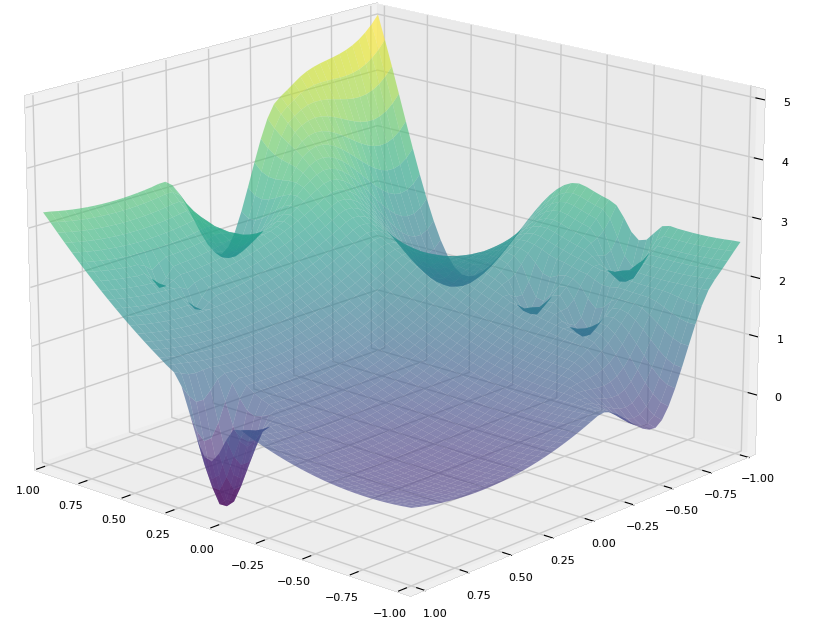
\includegraphics[width=1\linewidth]{figure/fig5.png}
			\caption{Graph of the benchmark objective function $\varphi(y)$} %% подпись к рисунку
			\label{fig:fig2}
		\end{minipage}
	\end{center}
\end{figure}	

\begin{figure}
	\begin{center}
		\begin{minipage}[h]{0.8\linewidth}
			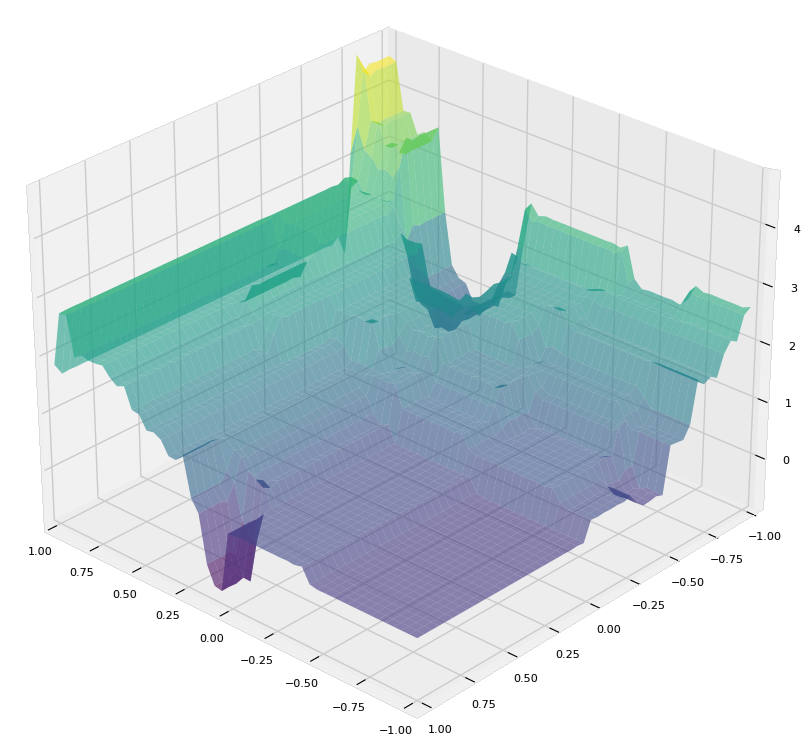
\includegraphics[width=1\linewidth]{figure/fig4.png}
			\caption{Graph of the piecewise-constant approximation $\psi(y)$ of the function $\varphi(y)$} %% подпись к рисунку
			\label{fig:fig2_2}
		\end{minipage}
	\end{center}
\end{figure}	


%При реализации алгоритма поиска областей притяжения локальных минимумов для построения дерева решений использовались алгоритмы из библиотеки OpenCV. OpenCV — это библиотека с открытым исходным кодом алгоритмов компьютерного зрения, обработки изображений и численных алгоритмов общего назначения. Более подробную информацию о дереве решений можно найти в \cite{Brahmbhatt2013}.
To implement the algorithm for identifying the regions of attraction for local minima to construct the decision tree algorithms from the OpenCV library were employed. OpenCV is an open-source library encompassing computer vision algorithms, image processing methods, and general-purpose numerical routines. Detailed information on decision trees may be found in \cite{Brahmbhatt2013}.


%После определения с помощью дерева решений области притяжения локального минимума, из точки ближайшего испытания, проведенного в этой области, запускается локальный метод. Мы использовали метод Хука--Дживса, который относится к классу методов нулевого порядка. Его правила вычисления представляют собой комбинацию исследовательского поиска (для выбора направления) и поиска в выбранном направлении \cite{Himmelblau72}.
Having identified a basin of attraction for a local minimum using the decision tree, a local method is launched from the nearest trial point conducted within that basin. We employed the Hooke-Jeeves method, classified as a zero-order technique. Its computational rules combine an exploratory search (for direction selection) with a search along the selected direction \cite{Himmelblau72}.


%%%%%%%%%%%%%%%%%%%%%%%%%%%%%%%%%%%%%%%%%%%%%%%%%%%%%%%%%%%%%%%%%%%%%%%%%%%%%%%%%%%%%%%%%
%%%%%%%%%%%%%%%%%%%%%%%%%%%%%%%%%%%%%%%%%%%%%%%%%%%%%%%%%%%%%%%%%%%%%%%%%%%%%%%%%%%%%%%%%
%%%%%%%%%%%%%%%%%%%%%%%%%%%%%%%%%%%%%%%%%%%%%%%%%%%%%%%%%%%%%%%%%%%%%%%%%%%%%%%%%%%%%%%%%

Исследующий поиск определяется следующим образом: 
\begin{itemize}[label=$\bullet$] 
	\item Определяется значение шага (он различен для каждого направления координат и может измениться во время поиска). 
	\item Шаг поиска считается успешным, если значение целевой функции в контрольной точке не превышает значение исходной целевой функции. 
	\item В противном случае нужно вернуться к предыдущему пункту и сделать шаг в обратном направлении. 
	\item После перебора всех N координат исследовательский поиск заканчивается. Полученная точка называется базовой точкой.
\end{itemize}
Поиск по образцу состоит из выполнения одного шага от полученной базовой точки вдоль линии, соединяющей ее с предыдущей базовой точкой.


%%%%%%%%%%%%%%%%%%%%%%%%%%%%%%%%%%%%%%%%%%%%%%%%%%%%%%%%%%%%%%%%%%%%%%%%%%%%%%%%%%%%%%%%%
%%%%%%%%%%%%%%%%%%%%%%%%%%%%%%%%%%%%%%%%%%%%%%%%%%%%%%%%%%%%%%%%%%%%%%%%%%%%%%%%%%%%%%%%%
%%%%%%%%%%%%%%%%%%%%%%%%%%%%%%%%%%%%%%%%%%%%%%%%%%%%%%%%%%%%%%%%%%%%%%%%%%%%%%%%%%%%%%%%%

\begin{figure} 
	\begin{center} 
		\begin{minipage}[h]{1.0\linewidth} 
			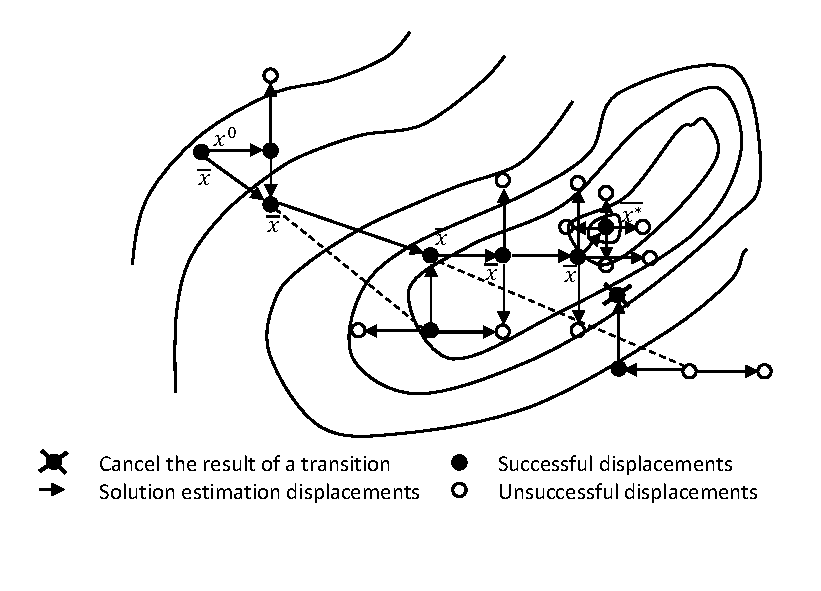
\includegraphics[width=1\linewidth]{figure/fig1.pdf} 
			\caption{An example showing the iterations of the Hooke-Jeeves method} %%  подпись к рисунку 
			\label{fig:fig1} 
		\end{minipage} 
	\end{center} 
\end{figure}	


Fig. \ref{fig:fig1} visually demonstrates the local algorithm in action. Level lines are shown with filled circles representing successful steps and open circles indicating unsuccessful steps from the exploratory search. 


\section{Global search algorithm with local methods starting in parallel}\label{SecGSA}

%TODO
%Здесь нужны общие слова про параллельную программу с несколькими процессами, мастером и рабочими

At the initial stage, the master process (let it have the identifier 0) launches $p$ trials in parallel at $p$ different points $\{y\left(x^1\right),y\left(x^2\right),\ldots,y\left(x^p\right)\}$, where preimages $\{x^1,x^2,\ldots,x^p\}$ are form the interval $[0,1]$.
Two preimages are the boundary points $x^1=0, x^p=1$; the remaining preimages are interior points $x^i\in\left(0,1\right),i=2,\ldots,p-1$.

Let us now assume that the algorithm has completed $K \geq 0$ iterations and $k \geq K$ trials have been performed.

%TODO
%Здесь нужно связующее предложение

\begin{enumerate}
	
	\item Извлекаем из множество $U$ (координат точек испытания) $c = max(p, |U|)$ координат точек испытания $y^{k+1}=y\left(x^{k+1}\right) ... y^{k+c}=y\left(x^{k+c}\right)$. Если $c < p$ то сначала вычисляем $n = p - c$ точек согласно шагам 2 - 7, иначе сразу переходим к шагу 8.	
	
	\item Перенумеруем (по нижними индексами) точки $x^i, 1\leq i\leq k$, а также граничные точки отрезка $[0,1]$ в порядке возрастания координаты  
	\begin{equation} 
		\label{agp1_sort} 	0=x_0<\ x_1<\ ...\ <x_{k+1}=1. 	
	\end{equation} 
	и сопоставить их со значениями $z_i=f(x_i)$. 
	
	\item  Вычислить текущую нижнюю оценку $M$ неизвестной константы Гельдера $H$: 
	\begin{equation} 
		\label{agp2_mu} 	\mu=max\left\{\frac{|z_i-z_{i-1}|}{{{(x}_i-x_{i-1})}^{1/N}},\ i=1,\ldots,k\right\},\ M=\  \left\{\begin{matrix}r\mu,\ \mu>0,\\1,\ \mu=0,\\\end{matrix}\right.\ 	
	\end{equation} 
	где $r>1$ — параметр алгоритма. Этот параметр управляет надежностью алгоритма: более высокие значения $r$ гарантируют гарантированное нахождение глобального минимума, выбор меньшего значения ускоряет сходимость алгоритма.
	
	\item  Для каждого интервала $(x_{i-1},x_i), 1\leq i\leq k+1,$ вычислить значение $R(i)$, называемое \textit{характеристикой} интервала, по формулам
	
	\begin{equation} 
		\label{agp3_R1} R(1)=2\Delta_1-4\dfrac{z_1}{M}, \; R(k+1)=2\Delta_{k+1}-4\dfrac{z_k}{M}, 
	\end{equation} 
	
	\begin{equation} 
		\label{agp3_Ri} R(i)=\Delta_i+\dfrac{(z_i-z_{i-1})^2}{M^2\Delta_i}-2\dfrac{z_i+z_{i-1}}{M},1<i<k+1, 
	\end{equation} 
	
	где \(\Delta_i=(x_i-x_{i-1})^\frac{1}{N}\).
	
	\item   Упорядочить характеристики $R\left(i\right),\ 1\leq i \leq k+1,$ в порядке не возрастания
	\begin{equation} 
		\label{agp4_R_sort} 	R\left(t_1\right)\geq\ R\left(t_2\right)\geq...\geq\ R\left(t_k\right)\geq\ R(t_{k+1}),\  
	\end{equation} 
	и выделить $n$ интервалов с индексами $t_j,\ 1\le\ j\le\ n$  с наибольшими значениями характеристик.	
	
	\item Вычислить новые координаты точки испытания $y'^{k+j}=y\left(x^{k+j}\right), \ 1\leq j\leq n$ прообразом которого является $x^{k+j}\in\left(x_{t_j-1},x_{t_j}\right)$, в соответствии с формулой
	\begin{equation}
		\label{agp5_x1}
		x^{k+1}=\frac{x_t+x_{t-1}}{2}-\mathrm{sign}\left(z_t-z_{t-1}\right)\frac{1}{2r}\left[\frac{\left|z_t-z_{t-1}\right|}{M}\right]^N.
	\end{equation}	
	
	
	\item Отправить на процесс $j, \ 1\leq j\leq n$ координату $y'^{k+1} ... y'^{k+n}$  и сообщаем процессу, что нужно произвести одиночное испытание.
	
	\item Отправить на процессы $h, \ 1\leq h\leq c$ координаты точек $y^{k+1} ... y^{k+c}$ и сообщаем процессу, что нужно запустить локальный метод.
	
	\item Получить со всех $p$ процессов значения испытаний и добавить их в поисковую информацию.
	
	\item Добавить точки испытаний $y'^{k+1}=y\left(x^{k+1}\right) ... y'^{k+n}=y\left(x^{k+т}\right)$ к множеству $V$.
	
	\item Если $k\ <\ 100 N$, перейти к шагу 1.
	
	
	\item Строим дерево решений по всей накопленной поисковой информации, получаем аппроксимирующую функцию $\psi(y)$.
	
	\item Если дерево решений используется впервые, постройте равномерную сетку
	\begin{displaymath} 
		Y'=\{ y'\in R^N:\ a_i\le y'_i \le b_i,\ 1\le i\le N \},
	\end{displaymath} 
	где количество узлов сетки является параметром метода.
	
	\item Вычислить кусочно постоянную аппроксимацию функции $\psi(y)$, по дереву решений : $Z' = \{ z'=  \psi(y'), y' \in Y'\}$
	
	\item Для всех точек $y'\in V$ найдите точки $y'_q$, ближайшие к $y'$,
	
	Если ни одна точка $y'_q$ не имеет меньшего значения, чем $y'_q$, поместить $y'$ в множество $U$
	
	Очистить множество $V$.
	
	\item Проверка критериев остановки
	
	
\end{enumerate}

Следующие $p$ испытания выполняются параллельно в точках $x^{k+j},\ 1\leq j\leq p$, вычисляемых по формуле (\ref{agp5_x1}). По завершении испытаний результаты этих испытаний сохраняются в базе поисковой информации, а алгоритм переходит к вычислению новых точек испытания.
Отметим, что, как правило, процесс испытания в прикладных оптимизационных задачах гораздо более затратный по вычислительным ресурсам по сравнению с вычислением координаты точки.

Алгоритм останавливается в том случае, если выполняется условие \(\Delta_{t_j} < \varepsilon\) хотя бы для одного значения $t_j,\ 1\le\ j\le\ p$, из (\ref{agp4_R_sort} ). Этот критерий остановки (наряду с обычным для итерационных методов критерием ограничения числа выполняемых итераций) используется в прикладных задачах оптимизации, в которых точка глобального минимума $y^*$ априори неизвестна.

При решении тестовых задач, в которых известна точка глобального минимума $y^*$, можно использовать критерий остановки и по попаданию в окрестность глобального минимума. В этом случае метод останавливается, если выполняется условие $\left\|y(x_{t_j})-\ y^\ast\right\| < \varepsilon$ для одного $t_j,\ 1\le\ j\le\ p$ из (\ref{agp4_R_sort}).

В качестве окончательной оценки глобального минимума рассматриваемой задачи берется значение 
\begin{equation} 
	f_k^*=\min_{1\leq i \leq k}f(x_i), \; x_k^*=arg \min_{1\leq i \leq k}f(x_i). 
\end{equation} 


Обоснование такого способа организации вычислений см. в \cite{Strongin2000,Barkalov2016}. Модификации с учетом наличия ограничений-неравенств, а также информация о производной целевой функции представлены в \cite{Barkalov2002, Gergel1997, Barkalov2023, Gegrel2021}.





% переводить до этого раздела
\section{Numerical experiments}\label{SecR}

%Численные эксперименты проводились на суперкомпьютере Лобачевский. Каждый узел имел по два процессора Intel Sandy Bridge E5-2660 2,2 ГГц, 64 Гб оперативной памяти.
Numerical experiments were conducted on the Lobachevsky supercomputer. Each supercomputer node had two Intel Sandy Bridge E5-2660 2.2 GHz processors and 64 GB of RAM.

%В экспериментах использовался генератор тестовых задач GKLS, который может генерировать задачи многоэкстремальной оптимизации с известными свойствами: точка глобального минимума, количество локальных минимумов и др.
The GKLS test problem generator was used in the experiments. This generator can create multi-extremal optimization problems with known properties, such as the location of the global minimum, the number of local minima, etc.

%Ниже представлены результаты работы синхронного параллельного алгоритма глобального поиска  с использованием дерева решений для нахождения областей притяжения локальных минимумов. Численное сравнение проводилось на двух классах функций GKLS (Simple и Hard из \cite{Sergeyev2006}) размерностей 2, 3, 4 и 5. Эти два класса отличаются размером области притяжения точки глобального минимума. Для простого класса задач радиус области притяжения в три раза больше, чем для сложного.

The results below show the performance of a synchronous parallel global search algorithm using a decision tree to find basins of attraction for local minima. The numerical comparison was performed on two classes of GKLS functions (Simple and Hard from \cite{Sergeyev2006}) with dimensions 2, 3, 4, and 5. These two classes differ in the size of the basin of attraction for the global minimum. The simple class of problems has a radius of attraction that is three times larger than that of the hard class.

%%%%%%%%%%%%%%%%%%%%%%%%%%%%%%%%%%%%%%%%%%%%%%%%%%%%%%%%%%%%%%%%%%%%%%%%%%%%%%%%%%%%%%%%%
%%%%%%%%%%%%%%%%%%%%%%%%%%%%%%%%%%%%%%%%%%%%%%%%%%%%%%%%%%%%%%%%%%%%%%%%%%%%%%%%%%%%%%%%%
%%%%%%%%%%%%%%%%%%%%%%%%%%%%%%%%%%%%%%%%%%%%%%%%%%%%%%%%%%%%%%%%%%%%%%%%%%%%%%%%%%%%%%%%%


Критерием остановки алгоритмов было попадание очередных точек испытания в $\varepsilon$-близость к истинному глобальному минимуму. В таблицах \ref{tab:1} и \ref{tab:2} приведено среднее время решения и ускорение по времени относительно последовательного запуска, выполняемых алгоритмами при решении задач оптимизации. На рис. \ref{fig:fig4} приведено ускорение по числу итераций. Распараллеливание выполнено с использованием технологии MPI, эксперименты проводились на 1, 8, 16, 32 и 64 процессах.


\begin{table}[!ht]
	\caption{Среднее время решения}
	\label{tab:1}
	\centering	
	\begin{tabular}{|l|l|l|l|l|l|}
		\hline
		2 & 1 mpi & 8 mpi & 16 mpi & 32 mpi & 64 mpi  \\ \hline
		hard & 12,71 & 1,98 & 1,71 & 0,87 & 1,65  \\ \hline
		simple & 6,35 & 0,57 & 1,27 & 0,95 & 0,21  \\ \hline
		3 & ~ & ~ & ~ & ~ &  \\ \hline
		hard & 14,19 & 5,59 & 2,10 & 0,75 & 0,60  \\ \hline
		simple & 5,92 & 1,63 & 1,17 & 0,38 & 0,41  \\ \hline
		4 & ~ & ~ & ~ & ~ &   \\ \hline
		hard & 66,29 & 34,93 & 8,53 & 4,95 & 2,93  \\ \hline
		simple & 31,88 & 9,44 & 4,71 & 4,67 & 5,51  \\ \hline
		5 & ~ & ~ & ~ & ~ &  \\ \hline
		hard & 324,04 & 52,42 & 17,55 & 11,48 & 10,60 \\ \hline
		simple & 53,77 & 6,62 & 3,38 & 1,99 & 1,70  \\ \hline
	\end{tabular}
\end{table}


\begin{table}[!ht]
	\caption{Ускорение по времени}
	\label{tab:2}
	\centering	
	\begin{tabular}{|l|l|l|l|l|}
		\hline
		2 & 8 mpi & 16 mpi & 32 mpi & 64 mpi  \\ \hline
		hard & 6,42 & 7,43 & 16,45 & 7,70  \\ \hline
		simple & 11,19 & 5,018 & 13,59 & 30,42  \\ \hline
		3 & ~ & ~ & ~ &   \\ \hline
		hard & 4,01 & 6,76 & 22,41 & 23,48  \\ \hline
		simple & 3,98 & 5,07 & 14,97 & 14,49  \\ \hline
		4 & ~ & ~ & ~ &   \\ \hline
		hard & 3,52 & 7,77 & 15,64 & 22,61  \\ \hline
		simple & 4,20 & 6,77 & 7,27 & 5,79  \\ \hline
		5 & ~ & ~ & ~ &   \\ \hline
		hard & 10,28 & 18,46 & 38,76 & 30,57  \\ \hline
		simple & 10,80 & 15,93 & 31,96 & 31,65  \\ \hline
	\end{tabular}
\end{table}


%\begin{table}[!ht]
%	\caption{Ускорениепо итерациям}
%	\label{tab:3}
%	\centering	
%	\begin{tabular}{|l|l|l|l|l|}
	%		\hline
	%		2 & 8 mpi & 16 mpi & 32 mpi & 64 mpi  \\ \hline
	%		hard & 37,61 & 49,11 & 50,04 & 34,58  \\ \hline
	%		simple & 52,06 & 19,72 & 63,02 & 307,59  \\ \hline
	%		3 & ~ & ~ & ~ &   \\ \hline
	%		hard & 15,03 & 92,04 & 47,28 & 89,74  \\ \hline
	%		simple & 10,25 & 44,70 & 44,29 & 76,87  \\ \hline
	%		4 & ~ & ~ & ~ &   \\ \hline
	%		hard & 38,14 & 106,64 & 58,40 & 117,56  \\ \hline
	%		simple & 30,75 & 79,84 & 29,41 & 40,43  \\ \hline
	%		5 & ~ & ~ & ~ &   \\ \hline
	%		hard & 162,66 & 269,09 & 201,95 & 206,94  \\ \hline
	%		simple & 46,13 & 176,70 & 98,42 & 191,00  \\ \hline
	%	\end{tabular}
%\end{table}



\begin{figure} 
	\begin{center} 
		\begin{minipage}[h]{0.9\linewidth} 
			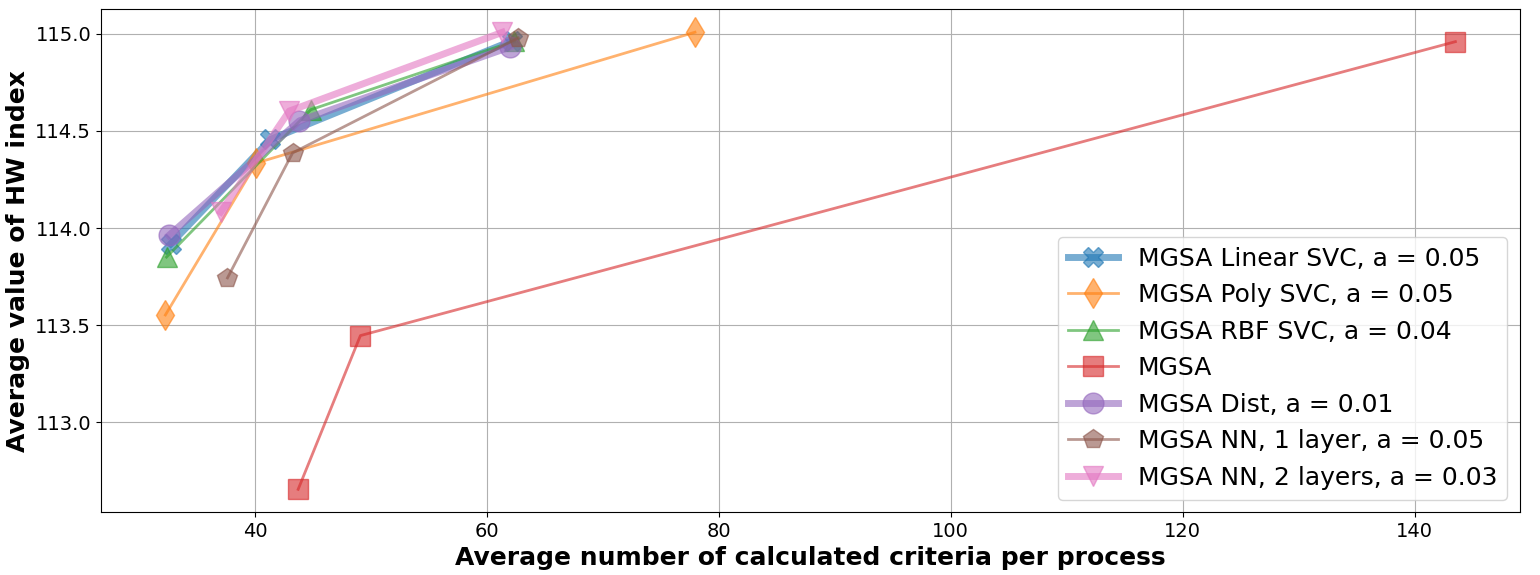
\includegraphics[width=1\linewidth]{figure/fig6.pdf} 
			\caption{Ускорение по итерациям} %%  подпись к рисунку 
			\label{fig:fig4} 
		\end{minipage} 
	\end{center} 
\end{figure}	


Как видно из приведенных данных, присутствует ускорение по времени для задач любой размерности, при этом в целом значение ускорения не линейное, но встречается и сверхлинейное ускорение. В данных задачах большое значение имеет что, как быстро алгоритм глобального поиска поставит достаточное для дерева решения количество точек в окрестности глобального минимума, после чего локальный метод быстро находит оптимум, из за этого возникает сверхлинейное ускорение. Низкое ускорение в остальных случаях, в большей степени обусловлено тем, что алгоритм оптимизации является синхронным и на некоторых итерациях происходит ожидание завершения локального поиска, также значительным оказалось влияние накладных расходов на передачу точек между процессами. 


%%%%%%%%%%%%%%%%%%%%%%%%%%%%%%%%%%%%%%%%%%%%%%%%%%%%%%%%%%%%%%%%%%%%%%%%%%%%%%%%%%%%%%%%%
%%%%%%%%%%%%%%%%%%%%%%%%%%%%%%%%%%%%%%%%%%%%%%%%%%%%%%%%%%%%%%%%%%%%%%%%%%%%%%%%%%%%%%%%%
%%%%%%%%%%%%%%%%%%%%%%%%%%%%%%%%%%%%%%%%%%%%%%%%%%%%%%%%%%%%%%%%%%%%%%%%%%%%%%%%%%%%%%%%%







\section{Conclusion} 

На данный момент в результате проделанной работы удалось совместить алгоритм глобального поиска с методом локальной оптимизации. В отличие от известных многозаходных схем решение о запуске локального метода принимается с помощью дерева решений. Использование такой комбинации методов позволяет значительно ускорить работу алгоритма.

Параллельная версия алгоритма сохраняет свойства своего последовательного прототипа, что было подтверждено численными экспериментами по решению серии из нескольких сотен задач различной размерности. Предлагаемая схема позволяет использовать преимущества как распараллеливания, так и быстрого поиска локальных экстремумов.

Помимо использования деревьев решений для выявления областей притяжения локальных экстремумов многоэкстремальных функций, мы также планируем использовать методы машинного обучения для разделения переменных решаемой задачи. Во многих прикладных задачах оптимизации зависимость целевой функции от некоторых параметров бывает либо линейной, либо одномодальной. Выделение таких переменных в специальную группу и решение задачи с помощью параллельной схемы рекурсивной оптимизации \cite{Barkalov2020_1} позволяет сократить время решения задачи на порядки по сравнению с использованием глобального поиска сразу по всем переменным.

%%%%%%%%%%%%%%%%%%%%%%%%%%%%%%%%%%%%%%%%%%%%%%%%%%%%%%%%%%%%%%%%%%%%%%%%%%%%%%%%%%%%%%%%%
%%%%%%%%%%%%%%%%%%%%%%%%%%%%%%%%%%%%%%%%%%%%%%%%%%%%%%%%%%%%%%%%%%%%%%%%%%%%%%%%%%%%%%%%%
%%%%%%%%%%%%%%%%%%%%%%%%%%%%%%%%%%%%%%%%%%%%%%%%%%%%%%%%%%%%%%%%%%%%%%%%%%%%%%%%%%%%%%%%%


\begin{credits}
	\subsubsection{\ackname} A bold run-in heading in small font size at the end of the paper is
	used for general acknowledgments, for example: This study was funded
	by X (grant number Y).
	
	\subsubsection{\discintname}
	The authors have no competing interests to declare that are
	relevant to the content of this article.
\end{credits}

%%%%%%%%%%%%%%%%%%%%%%%%%%%%%%%%%%%%%%%%%%%%%%%%%%%%%%%%%%%%%%%%%%%%%%%%%%%%%%%%%%%%%%%%%
%%%%%%%%%%%%%%%%%%%%%%%%%%%%%%%%%%%%%%%%%%%%%%%%%%%%%%%%%%%%%%%%%%%%%%%%%%%%%%%%%%%%%%%%%
%%%%%%%%%%%%%%%%%%%%%%%%%%%%%%%%%%%%%%%%%%%%%%%%%%%%%%%%%%%%%%%%%%%%%%%%%%%%%%%%%%%%%%%%%


%
% ---- Bibliography ----
%
\bibliographystyle{spmpsci}
\bibliography{bibliography}{}











\end{document}
